\color{black}
{\color{secblue}\subsection{Product perspective}}
The following class diagram sums up conceptually the system behind the services Data4Help, AutomatedSOS and Track4Run.
\begin{figure}[H]
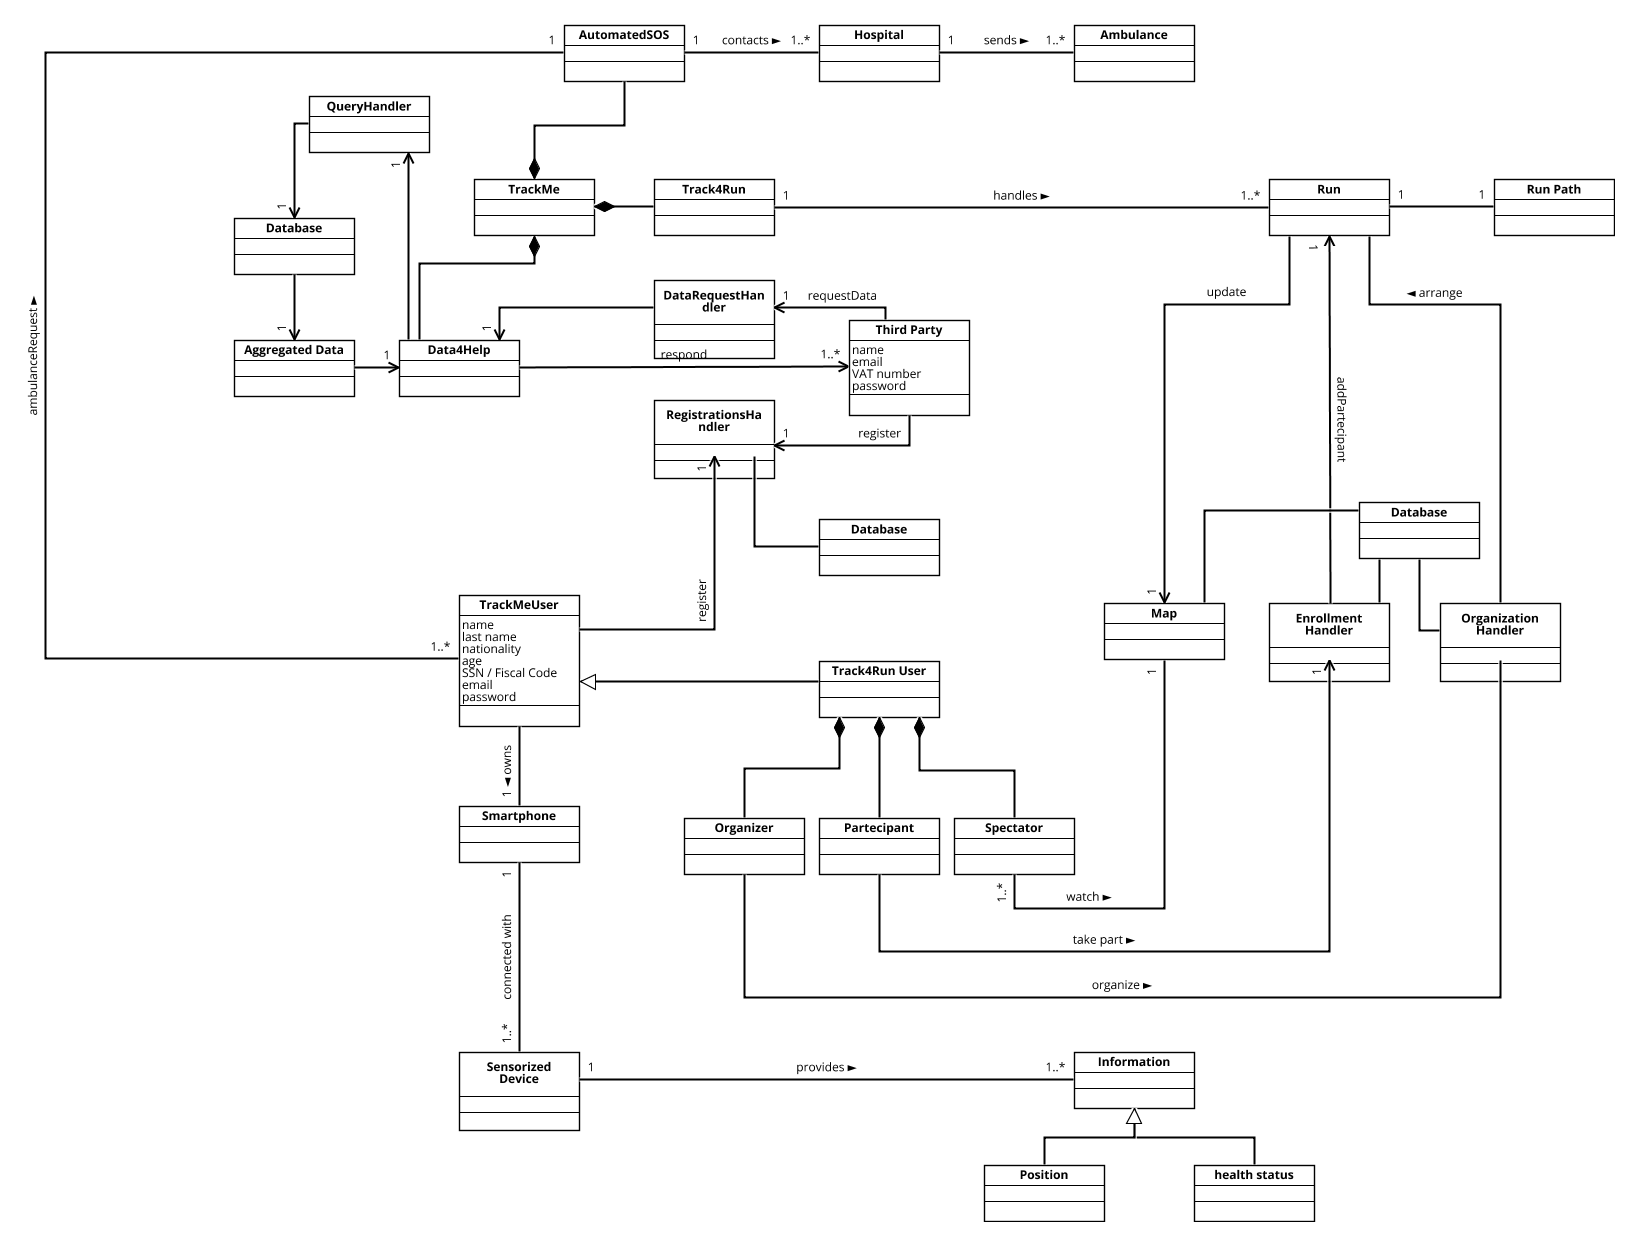
\includegraphics[width=\linewidth]{./Images/RASD_UML.png}
\centering
\caption{UML diagram}
\end{figure}
From this diagram it's visible that for the three services only one TrackMe account is needed to be created.
The class TrackMe is mainly a container of the three services.
Database is only one class, it gets repetead more than once only to make the diagram clearer to be looked at.

\newpage
Here will follow the state diagrams of each of the services provided by TrackMe.

\begin{figure}[H]
    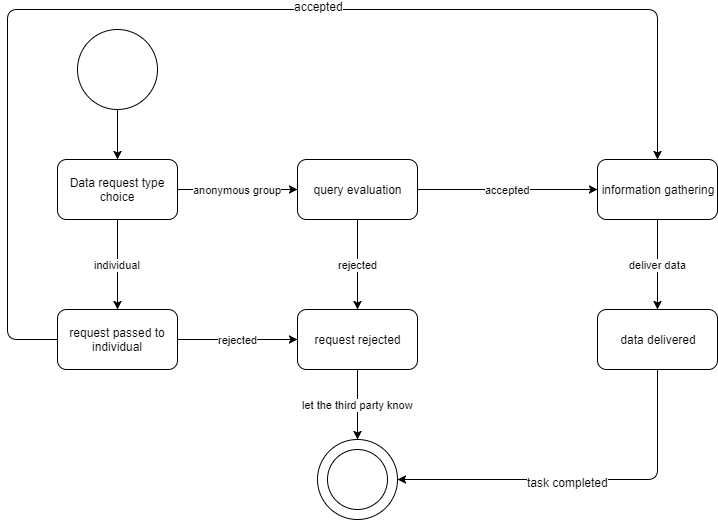
\includegraphics[width=\linewidth]{./Images/RASD_State_Diagram.png}
    \centering
    \caption{Data4Help state diagram}
  \end{figure}
  
  
  \begin{figure}[H]
    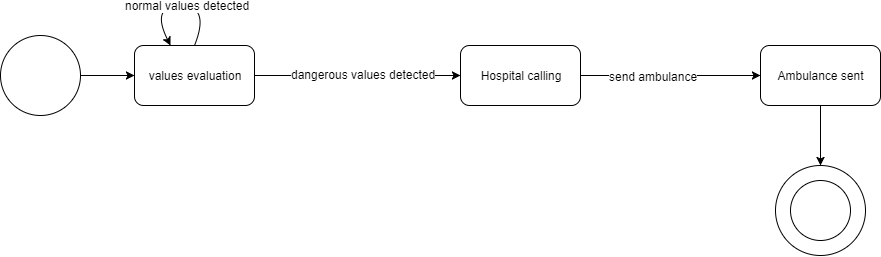
\includegraphics[width=\linewidth]{./Images/Automated_SOS_state_diagram.png}
    \centering
    \caption{AutomatedSOS state diagram}
  \end{figure}


 \begin{figure}[H]
    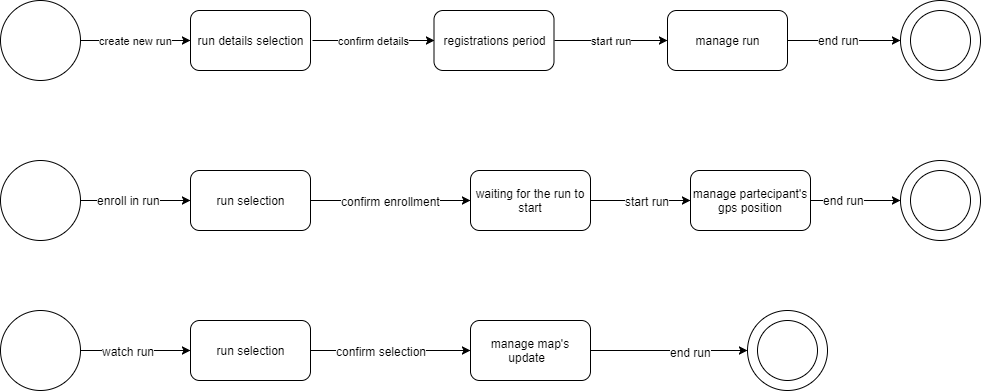
\includegraphics[width=\linewidth]{./Images/Track4Run_state_diagram.png}
    \centering
    \caption{Track4Run state diagram}
  \end{figure}

{\color{secblue}\subsection{Product functions}}
\begin{itemize}
\item The first essential requirement is that all the data must be available remotely for all registered third parties;
\item The second essential requirement is that all the data must be available in a anonymized way, so that no third parties can trace back a specific user data;
\item The third essential requirement is high reliability for the AutomatedSOS service, because of its nature: the service must automatically detect an emergency and act accordingly without the user's interaction. It must be also active 24/7, must have low time response, and must be connected with an automated emergency call service;
\item The fourth essential requirement for the Track4Run service is to be scalable enough for managing any number of active users simultaneously;
\item The fifth essential requirement is that third parties users can have access to all the data from a specific user if that user allow them to do so;
\item The sixth essential requirement is that third parties users can register to a query that was previously requested;
\end{itemize}
{\color{secblue}\subsection{User characteristics}}
Relevant information for each actor:
\begin{itemize}
\item Data4Help Users: these users don't require specific needs, as they only passively contribute to the acquisition of general data for the use of third-parties. Only a smartphone and a smartwatch, or similar device, is required for these users.
\item Registered Third-parties to Data4Help: their need is to be able to acquire various aggregated type of data, filtering their requests based on one or more parameter of the users, like location, personal informations etc. They must receive an answer if the number of results is not too low. Also all answers are anonymized.
\item Users of AutomatedSOS: their need is an application always online which constantly checks their health status and in case of emergency automatically calls an ambulance for them.
\item Users of Track4Run: these users must be able to create a specific track, to browse the available ones, and to join in one or more of them. This user must also be able to be tracked by their position during the run. Also, users that have created a run can join as a partecipant or a spectator as they like.
\end{itemize}
{\color{secblue}\subsection{Assumptions, dependencies and constraints}}
\begin{itemize}
\item D1 - Every user of Data4Help has a smartwatch or a compatible wearable device.
\item D2 - Data acquired through the users' devices is correct and not manipulated.
\item D3 - An automatic ambulance calling service exists. Once the nearest hospital is localized by the system, such service gets called.
\item D4 - The application has access to the ambulance calling system.
\item D5 - The position acquired for tracking each Track4Run's runner is accurate enough, which means that the GPS system needs to be able to track users in a 5 meters diameter.
\end{itemize}